\section{Daten und Portfolio-Vorbereitung}

Im Rahmen dieses Kapitels wird die Methodik zur Generierung eines repräsentativen Musterportfolios erläutert, das als Grundlage für die Prognose klimabedingter Schäden dient. Trotz des umfangreichen Datenbestands der Finanzinstitute über ihre Kreditengagements hat die limitierte Zugänglichkeit zu detaillierten Datensätzen bisher umfassende empirische Analysen der Kreditrisiken eingeschränkt. Zur Überwindung dieser Limitation wird ein Musterportfolio konstruiert, das eine fundierte Approximation der erwarteten Verluste aus Wohnimmobilienkrediten ermöglicht. Die Quantifizierung essenzieller Risikoparameter basiert primär auf dem Geschäftsbericht der Münchener Hypothekenbank \parencite{MuenchenerHyp2022}, ergänzt durch ausdifferenzierte Datensätze zur Distribution von Energieeffizienzklassen und regionalen Verteilung von Wohneinheiten. Diese Datenaggregation bildet die Basis für eine detaillierte Analyse der Anfälligkeit verschiedener Immobilienarten und Standorte gegenüber umweltbedingten Wertänderungen, physischen Risiken sowie Transitionsrisiken.

Zum Stichtag 31.12.2023 belief sich der ausstehende Bestand an Wohnimmobilienfinanzierungen im Portfolio der Münchener Hypothekenbank in Bayern auf 8.921.489.311,00 €, wobei die durchschnittliche Größe der Darlehen für Wohnimmobilien circa 163.700,00 € betrug. Zur Ermittlung der Anzahl der Darlehen im Portfolio wird zunächst der Gesamtbestand durch die durchschnittliche Größe der Darlehen dividiert, was auf etwa 54.500 Darlehen schließen lässt. Unter Anwendung der Gleichung \ref{eq:cochran} zur Berechnung der erforderlichen Stichprobengröße für das theoretische Szenario einer unendlichen Anzahl von Immobilien im Portfolio ergibt sich bei einem Konfidenzintervall von 99\% und einer Fehlermarge von 2\% ein notwendiger Stichprobenumfang von 4.147 Datenpunkten. Die in Gleichung \ref{eq:finite_population} präsentierte Formulierung für endliche Populationen führt jedoch zu einer Reduktion auf 3.853 Darlehen als erforderliche Stichprobengröße für Portfolios mit mehr als 54.500 Elementen.

Da die in den Geschäftsberichten ausgewiesenen Kreditbestände lediglich das Risikoexposure des Kreditinstituts reflektieren und nicht den realen Immobilienwert repräsentieren, ergibt sich die Notwendigkeit, den Property Value in Relation zum Gesamtrisikoexposure zu evaluieren.
Die Münchener Hypothekenbank hat in ihrem Jahresbericht die Verteilung des Beleihungsauslaufs in tabellarischer Form offengelegt (siehe Tabelle \ref{tab:beleihungsauslauf2023}). Darüber hinaus wurde ein durchschnittlicher Beleihungsauslauf von 54,1\% für die Wohnimmobilienfinanzierung angegeben.
Diese Informationen stellen die fundamentalen finanziellen Parameter dar, die für die Konstruktion eines repräsentativen Immobilienportfolios essenziell sind.

\begin{table}[htbp]
    \centering
    \caption{Verteilung des Beleihungsauslaufs im Wohnimmobilienportfolio der Münchener Hypothekenbank zum 31.12.2023}
    \label{tab:beleihungsauslauf2023}
    \begin{tabularx}{\textwidth}{XXXXXXX}
    \toprule
    Beleihungsauslauf & bis 60\% & $>$60-70\% & $>$70-80\% & $>$80-90\% & $>$90-100\% & $>$100\% \\
    \midrule
    Prozentanteil & 39,2\% & 15,0\% & 16,4\% & 10,2\% & 8,2\% & 11,0\% \\
    \bottomrule
    \end{tabularx}
\end{table}

Der nächste Schritt beinhaltet die Erzeugung präziser Koordinaten für die Datenpunkte. Eine zufällige Verteilung von Punkten in Bayern würde die tatsächliche Struktur eines Kreditportfolios nicht angemessen widerspiegeln, da Immobilien sowohl in Deutschland als auch in Bayern ungleichmäßig verteilt sind. Die Studie von \textcite{zurek2022real} untersucht den Zusammenhang zwischen Bevölkerungsdichte und Kreditvergabe im deutschen Kontext. Sie unterstützt die Annahme, dass Gebiete mit stärkerem Wirtschaftswachstum - oft gekennzeichnet durch höhere Bevölkerungsdichte - zu höheren Immobilienpreisen und folglich zu einer erhöhten Kreditnachfrage neigen. Daher wird die Bevölkerungsdichte als Basis für die Zuweisung spezifischer Koordinaten zu jedem Datenpunkt verwendet.

Die von der Webseite \parencite{suche_postleitzahl} bereitgestellte Datengrundlage integriert geographische Rohdaten aus OpenStreetMap mit den offiziellen Ermittlungen der Bevölkerungszahlen durch die Statistischen Ämter des Bundes und der Länder. Diese Synthese ermöglicht eine präzise Segmentierung des Bundesgebiets in Postleitzahlenzonen, denen jeweils spezifische Bevölkerungskennzahlen zugeordnet sind.
Zur repräsentativen Verteilung der 3853 Datenpunkte, die der Anzahl der Hypothekarkredite entsprechen, wird ein proportionaler Ansatz basierend auf der Einwohnerzahl jeder Region angewandt. Innerhalb der jeweiligen Postleitzahlgebiete erfolgt die Platzierung mittels eines kontrollierten stochastischen Verfahrens, bei dem randomisierte Koordinaten generiert und auf ihre Lage innerhalb der definierten Polygongrenzen verifiziert werden. Dieses Vorgehen gewährleistet eine realitätsnahe räumliche Verteilung unter Berücksichtigung demographischer und geographischer Faktoren. Die resultierende Distribution der Datenpunkte ist in Abbildung \ref{fig:vergleich_bayern} visualisiert.

\begin{figure}[htbp]
    \centering
    \begin{subfigure}{\textwidth}
        \centering
        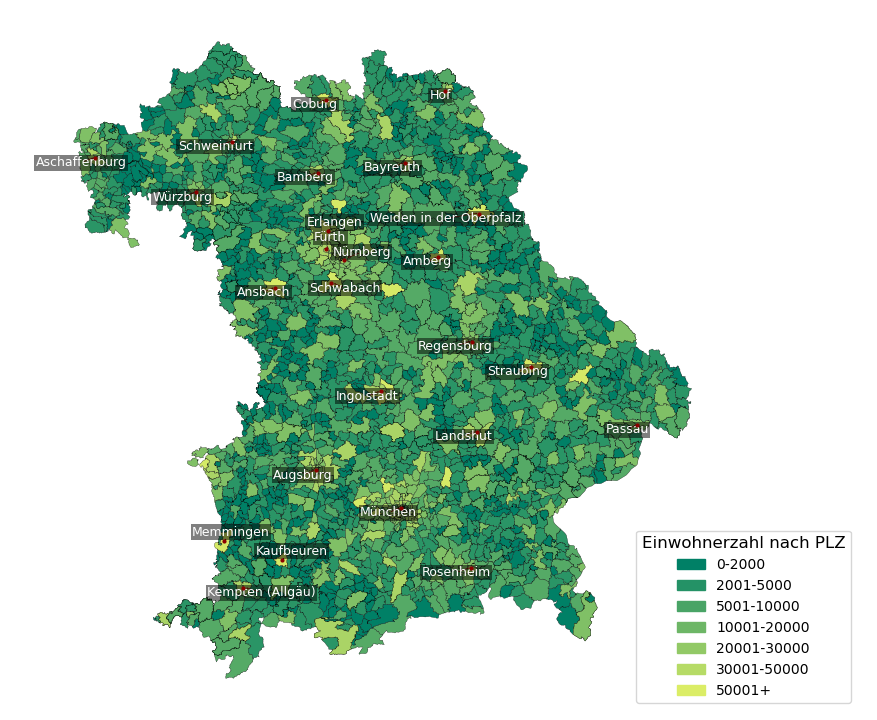
\includegraphics[width=0.8\textwidth]{figures/Bayern_pop_plz.png}
        \caption{Verteilung der Bevölkerungsdichte Bayerns nach Postleitzahlenbereichen}
        \label{fig:bevoelkerungsdichte}
    \end{subfigure}

    \vspace{1cm} % Fügt vertikalen Abstand zwischen den Bildern hinzu

    \begin{subfigure}{\textwidth}
        \centering
        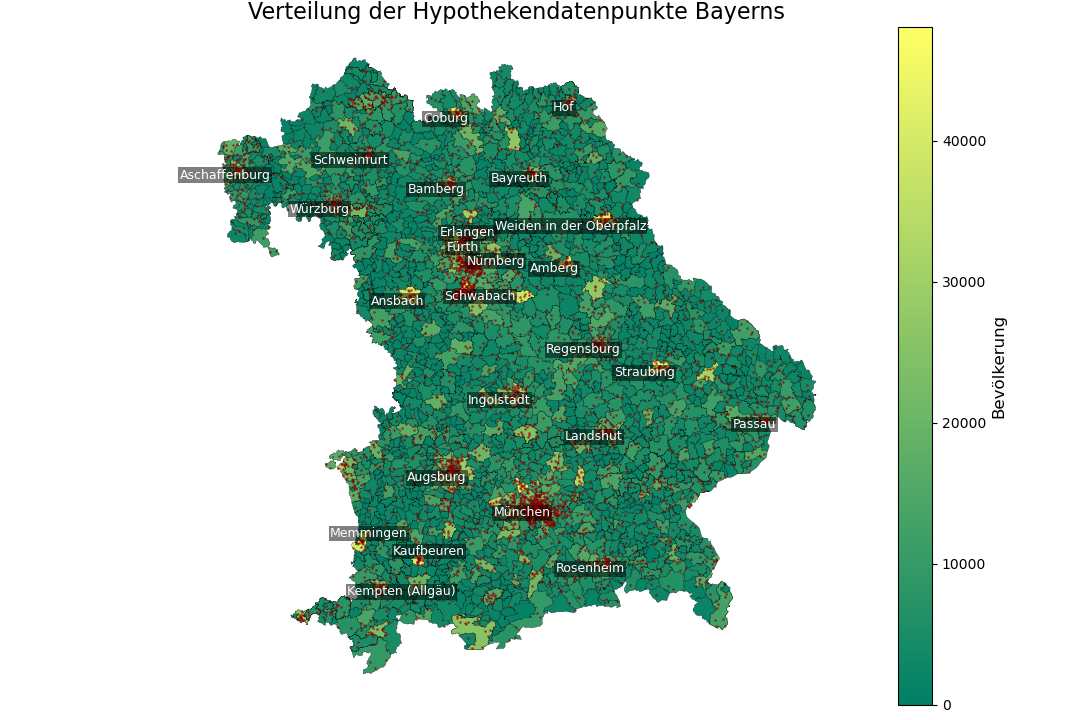
\includegraphics[width=0.8\textwidth]{figures/bayen_por_pop.png}
        \caption{Datenpunktverteilung im Hypothekenportfolio Bayern}
        \label{fig:hypothekenportfolio}
    \end{subfigure}
    \caption{Vergleich der Bevölkerungsdichte und der Hypothekenverteilung in Bayern}
    \label{fig:vergleich_bayern}
\end{figure}